\documentclass[fancy,11pt,twocol]{elegantbook}
\usepackage{booktabs}
\title{A Statistical Analysis of Age Prediction}
\subtitle{First Homework of Modern Biological Technology}

\author{Yufeng Xie}
\institute{School of Life Sciences, Tsinghua University}
\date{\today}
\version{1.0}

\extrainfo{}

\logo{i.png}
\cover{cov.pdf}

\begin{document}

\maketitle
\tableofcontents
\clearpage
\thispagestyle{empty}
\mainmatter
\hypersetup{pageanchor=true}

\chapter{Survey}
Prof.Wang taught Modern Biological Technology to graduate students. He made a survey about his age estimation. 
Of the 239 people, everyone submitted his own age, gender and age estimation.
Here are parts of the results:
% Table generated by Excel2LaTeX from sheet 'Sheet1'
\begin{table}[htbp]
	\centering
	\caption{Age Estimation}
	  \begin{tabular}{ccc}
	  \toprule
	  sex   & age   & pred\_age \\
	  \midrule
	  F     & 21    & 43 \\
	  F     & 22    & 45 \\
	  M     & 23    & 40 \\
	  F     & 21    & 45 \\
	  F     & 22    & 45 \\
	  F     & 22    & 45 \\
	  F     & 26    & 46 \\
	  F     & 22    & 46 \\
	  M     & 22    & 50 \\
	  \bottomrule
	  \end{tabular}%
	\label{tab:addlabel}%
  \end{table}%
  

Contact Infos:
\begin{itemize}
	\item Email: \email{xyf19@mails.tsinghua.edu.cn}
\end{itemize}


\section{Students Age}
To have a better understanding the distribution of data, we have a quick look on age using Waffle Chart.
\begin{figure}[htbp]
	\centering
	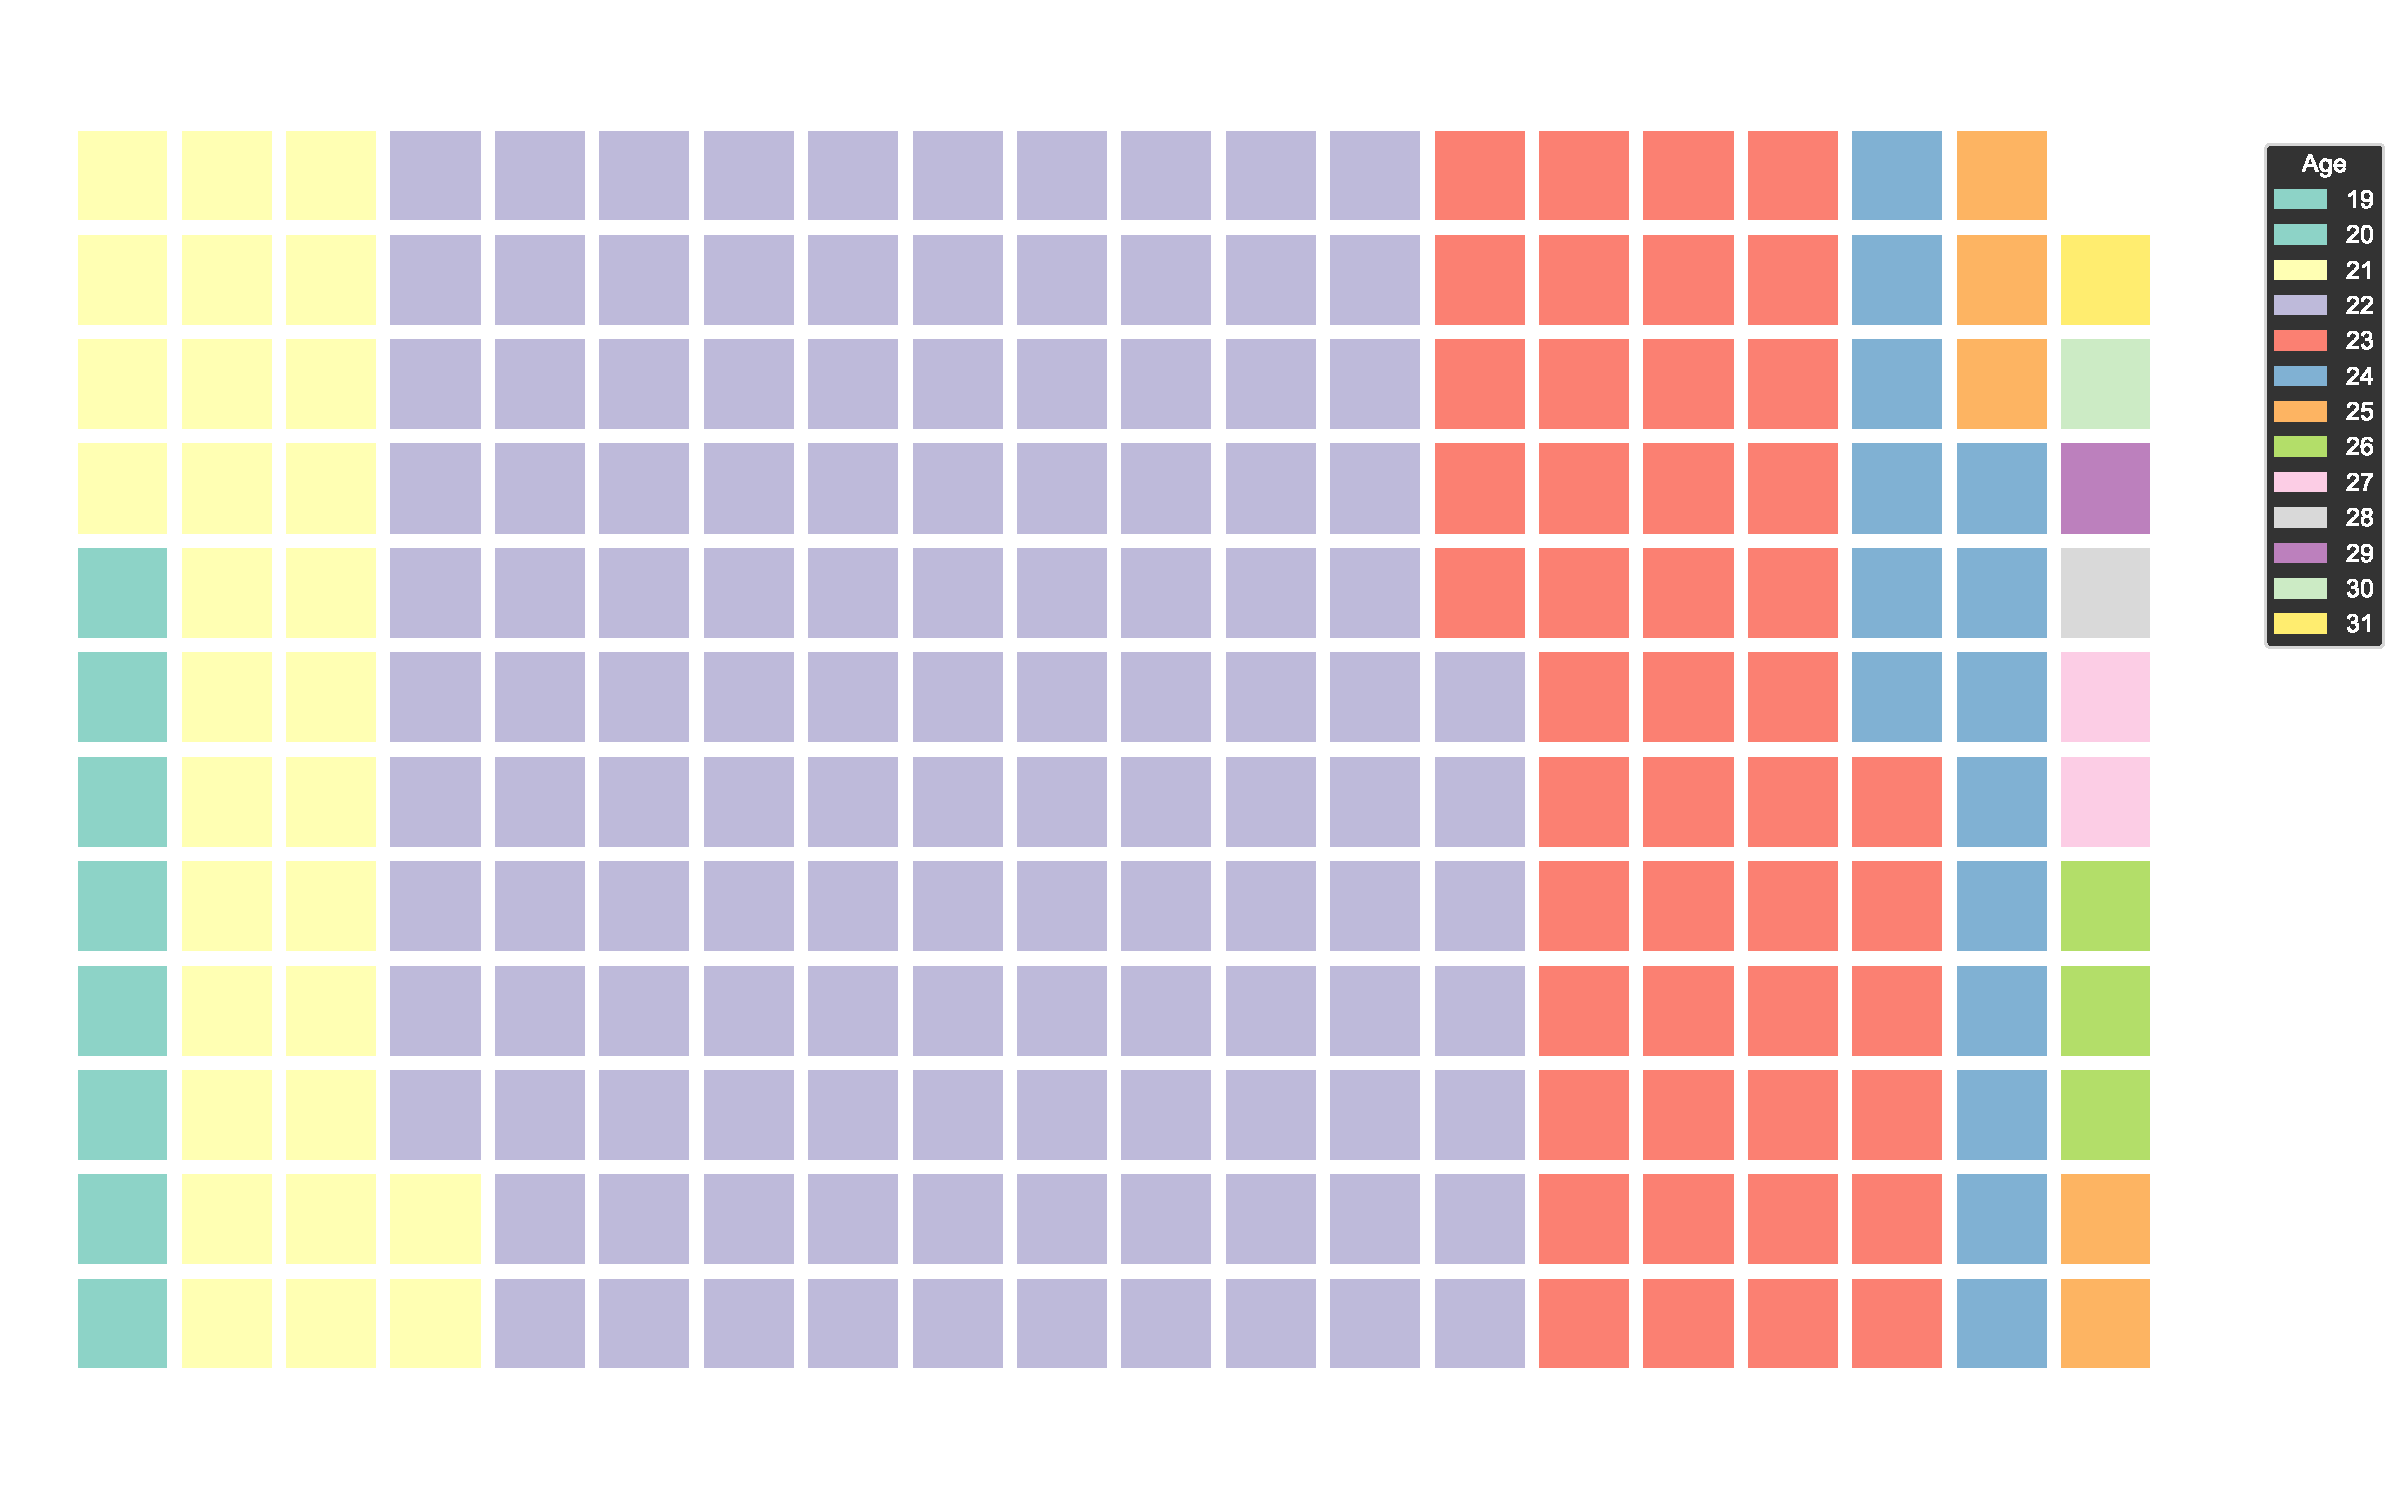
\includegraphics[width=0.7\textwidth]{waffe.pdf}
	\caption{Distribution of students' ages}
\end{figure}


\begin{note}
	Waffle chart, please refer to \href{https://en.wikipedia.org/wiki/Pie_chart#Square_chart_/_Waffle_chart}{this}.
\end{note}
Every cell represents one student. Most students are 22 and 23 years old.


\section{Students Age}
We have a quick look on gender using Waffle Chart.
\begin{figure}[htbp]
	\centering
	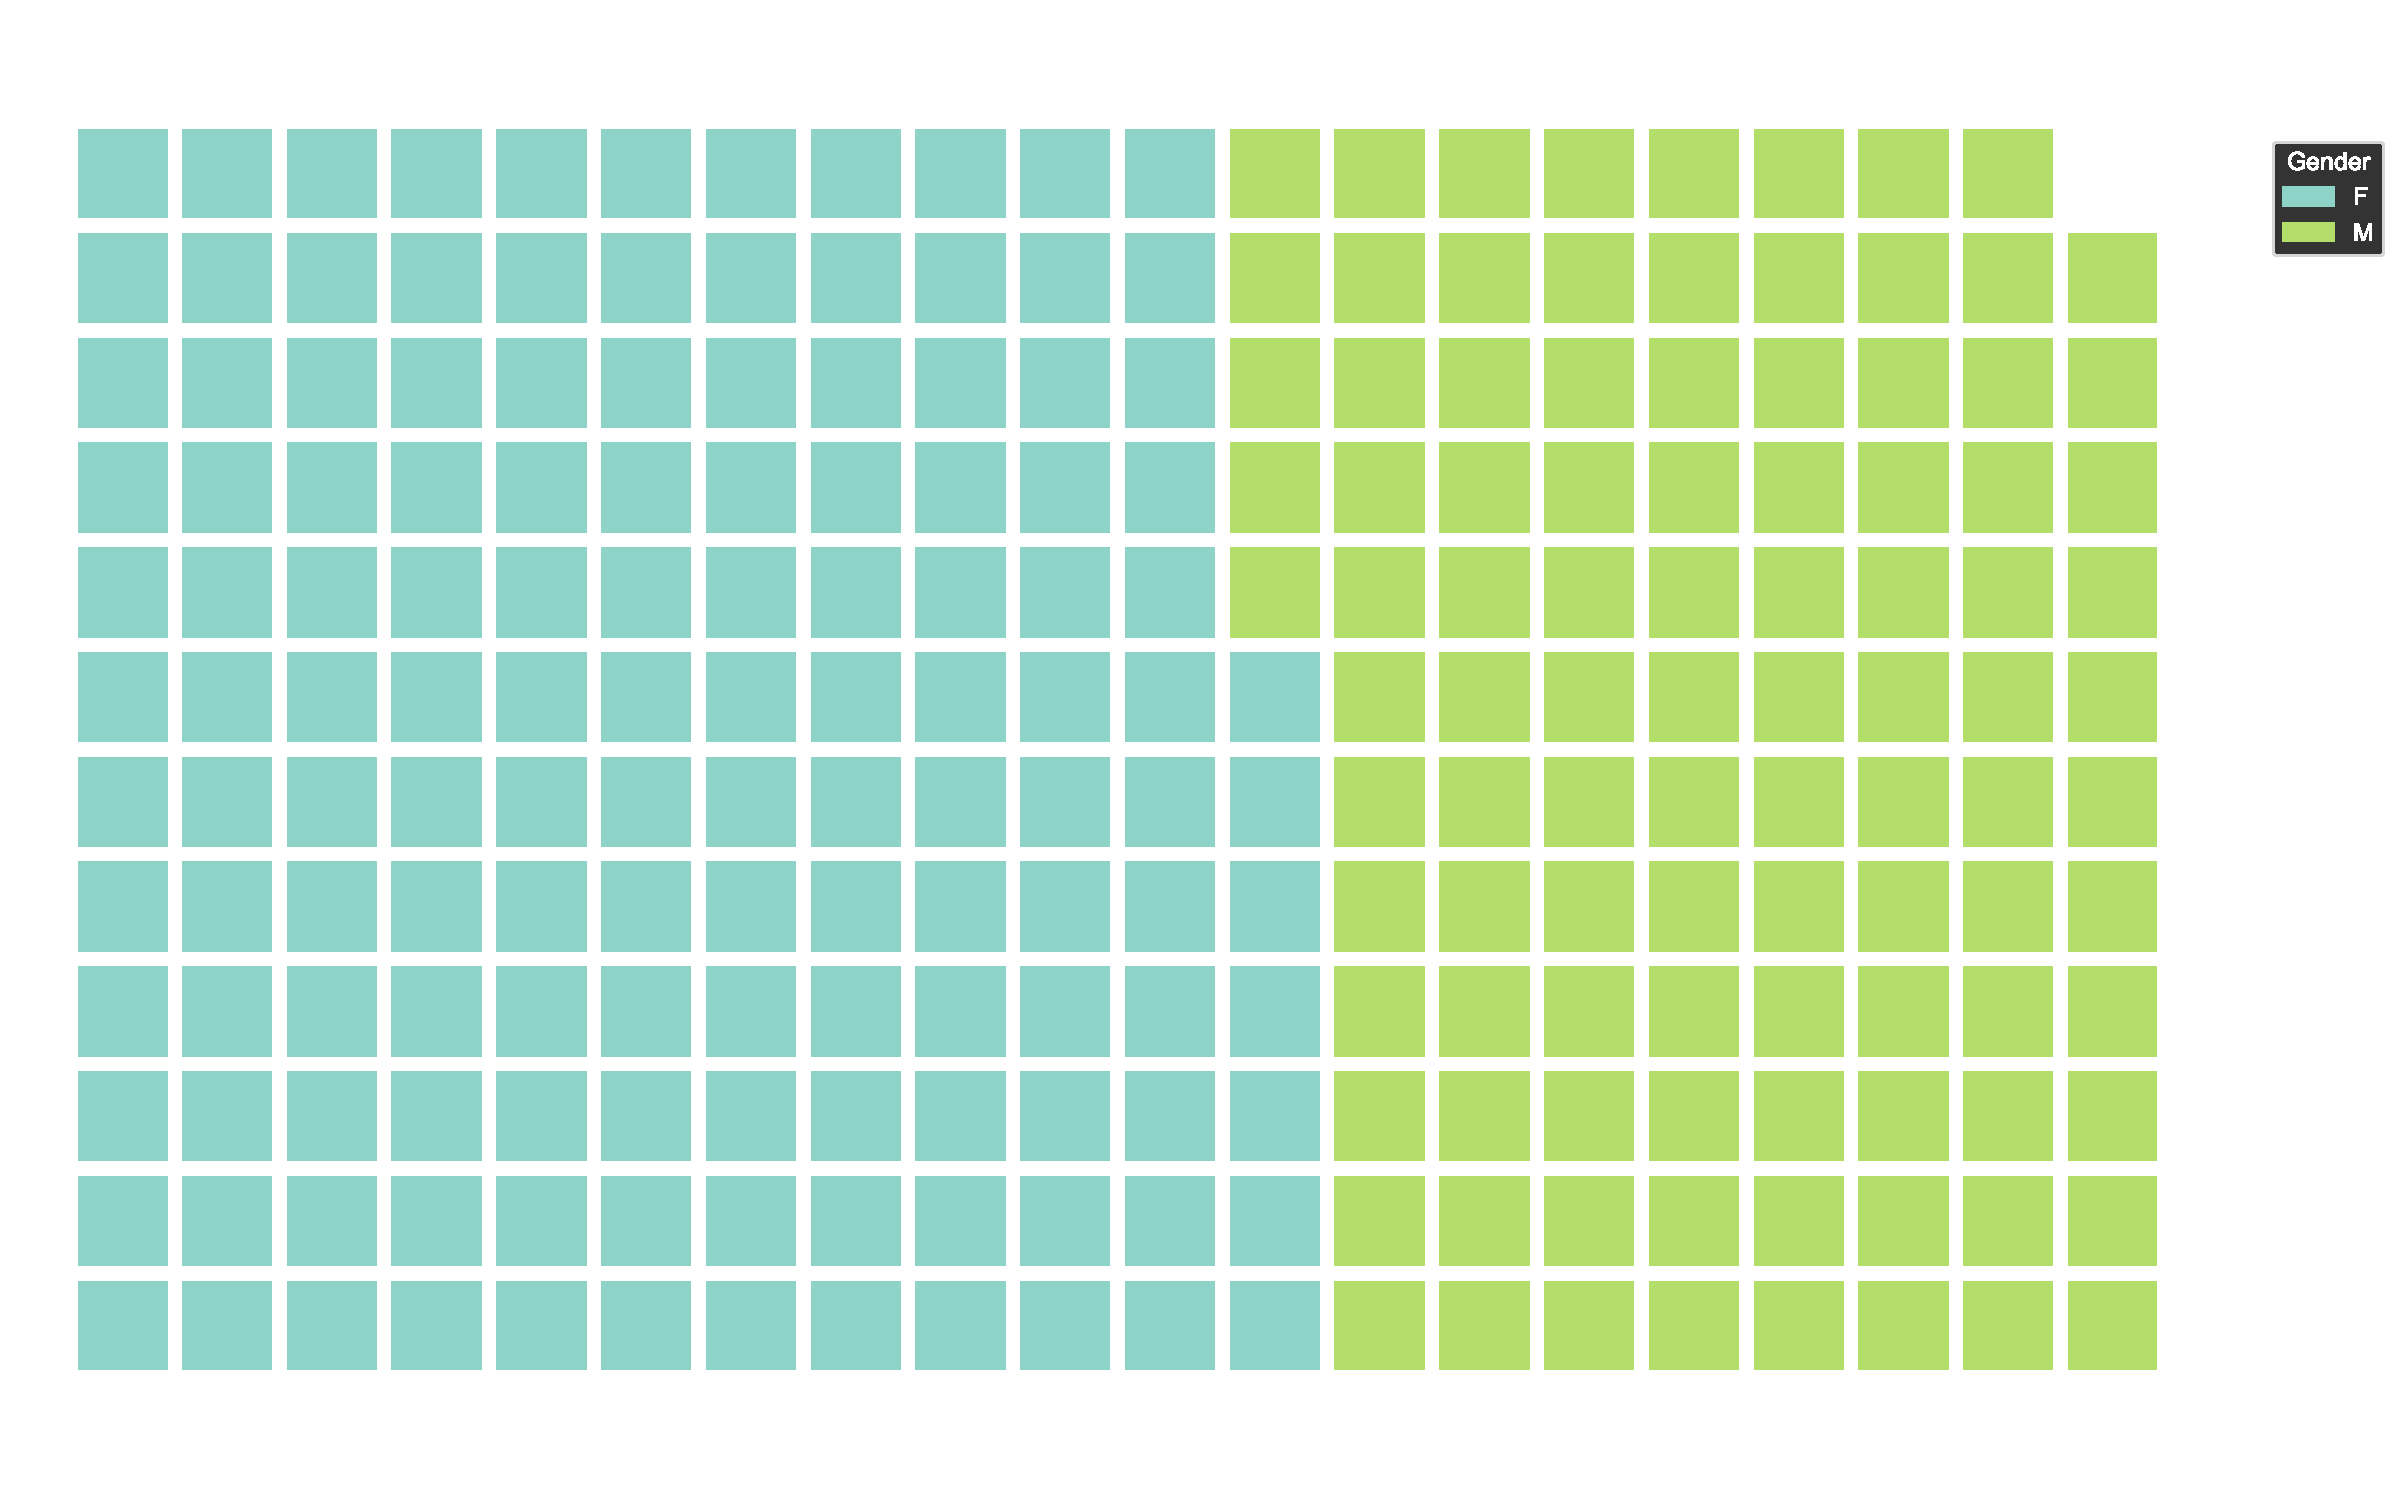
\includegraphics[width=0.7\textwidth]{waffle_sex.pdf}
	\caption{Distribution of students' genders}
\end{figure}


\chapter{The Normal Distribution}
To know whether age estimation obey normal distribution, we can have a graphic judgment or use nonparametric test method. 

\section{Normal Distribution Fit}
We plot the age estimation using histogram, and fit it with normal distribution. 
The data set is denoted as $A$, where $A_i$ represents an element and $i$ is a natural number from 1 to a total of 239.
We use $$
\frac{1}{n} \sum_{i=1}^{n} A_{i}
, n= 239$$ to estimate the average age, and adopt unbiased estimation of standard errors. 
$$
\frac{1}{n-1} \sum_{i=1}^{n}\left(A_{i}-\overline{A}\right)^{2}
$$
\begin{figure}[htbp]
	\centering
	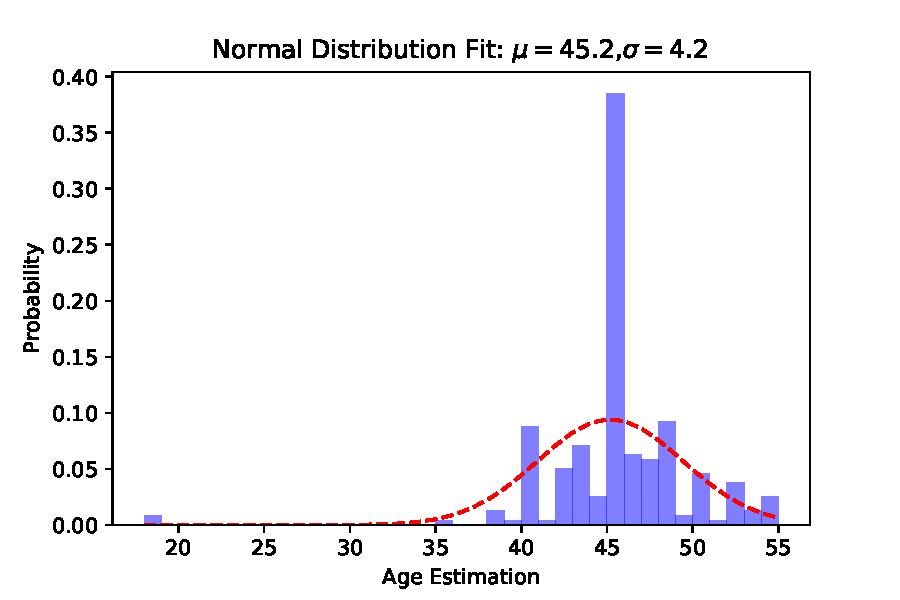
\includegraphics[width=0.7\textwidth]{norm_fit.pdf}
	\caption{The Fit of Age estimation distribution. 
	The x-axis represents the estimated age, 
	and the y-axis represents the proportion of people of the estimated age to the total number of people. 
	The purple histogram represents real data, and the red dotted line indicates the fit of the data. 
	The line is a normally distributed shape with $\mu$ and $\sigma$ being 45.2 and 4.2, respectively.  }
\end{figure}

We can see that most of the actual data is concentrated at an intermediate level, making it higher than the peak of the normal distribution. To 
There are two outliers. Two girls had the estimation to be 18.
\section{The quantitle-quantile plot}
\begin{introduction}
	\item The quantitle-quantile(q-q) plot is a graphical technique for determining if two data sets come from populations with a common distribution. If so, each data point has the same quantile in the two different data set, and the points should fall along the 45-degree reference line.
\end{introduction}

\begin{figure}[htbp]
	\centering
	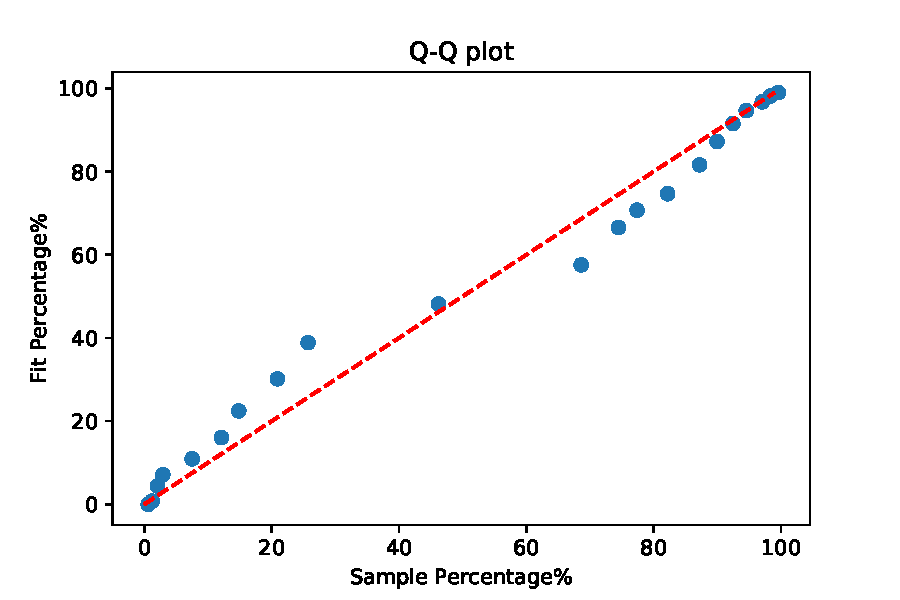
\includegraphics[width=0.7\textwidth]{qqplot.pdf}
	\caption{The quantitle-quantile plot of age estimation distribution. The points didn't fall along the $y=x$ reference line. }
\end{figure}

\begin{lstlisting}
	def qqplot(sample=raw['pred_age']):
		import numpy as np
		x = sample
		mu =np.mean(x)
		sigma =np.std(x,ddof=1)
		from scipy.stats import norm,percentileofscore
		samp_pct = [percentileofscore(x, i) for i in x]
		fit_pct = [norm.cdf(i,mu,sigma)*100 for i in x]
		import matplotlib.pyplot as plt
		plt.scatter(x=samp_pct, y=fit_pct)
		linex = np.arange(0, 100, 1)
		liney = np.arange(0, 100, 1)
		plt.plot(linex, liney, 'r--')
		plt.xlabel('Sample Percentage%') #绘制x轴 
		plt.ylabel('Fit Percentage%') #绘制y轴 
		plt.title(r'Q-Q plot')
		plt.savefig('qqplot.pdf')
	qqplot()
\end{lstlisting}

We compared the quantitles between age estimation dataset and standard normal distribution. The result may indicate that the data does not obey the normal distribution. We apply nonparametric test method to judge whether the data obey the normal distribution.





\section{Kolmogorov-Smirnov test}
Kolmogorov-Smirnov test is a nonparametric method to judge whether the data obey the normal distribution.
We are concerned about whether the data obey the normal distribution. Null hypothesis is that the data obey the normal distribution with $\mu$ and $\sigma$ being 45.2 and 4.2. Alternative hypothesis is that the data does't obey the normal distribution with $\mu$ and $\sigma$ being 45.2 and 4.2.
We test it with Python.

\begin{lstlisting}
import scipy.stats as stats
x = raw['pred_age']
mu =np.mean(x)
sigma =np.std(x,ddof=1)
normed_data=(x-mu)/sigma
print(stats.kstest(normed_data,'norm'))
\end{lstlisting}

The result is:
\begin{lstlisting}
KstestResult(statistic=0.2138458125325069, pvalue=4.5205350061342694e-10)
\end{lstlisting}
P-value is less than 0.05 and we can reject the null hypothesis, so the data doesn't obey the normal distribution.

To know whether the two girls affect the results, we delete their data, and have a test repeatly.
Null hypothesis is that after removing the two girls' data, the data obey the normal distribution.
Alternative hypothesis is that after removing the two girls' data, the data doesn't obey the normal distribution.
\begin{lstlisting}
	import scipy.stats as stats
	x = raw['pred_age']
	sp_x=x.tolist()
	sp_x.sort()
	sp_x = sp_x[2:]
	mu =np.mean(sp_x)
	sigma =np.std(sp_x,ddof=1)
	normed_data=(sp_x-mu)/sigma
	print(stats.kstest(normed_data,'norm'))
\end{lstlisting}
	
The result is:
\begin{lstlisting}
	KstestResult(statistic=0.19918782897725168, pvalue=1.0219734444990697e-08)
\end{lstlisting}
P-value is less than 0.05 and we can reject the null hypothesis, so the data doesn't obey the normal distribution.



\chapter{Gender}
We care about the influence of genders. For example, for the student of some gender, estimation of age is deeply affected by experience, so the data has a strong heterogeneity.
To know whether genders bring heterogeneity, we have Kolmogorov-Smirnov test on data of each gender.
\section{Male}
We individually had a test on mens' data to judge whether obeying the normal distribution.
Null hypothesis is that the mens' data obey the normal distribution.
Alternative hypothesis is that the mens' data doesn't obey the normal distribution.
\begin{lstlisting}
import scipy.stats as stats
	x = raw[raw['sex']=='M']['pred_age']
	mu =np.mean(x)
	sigma =np.std(x,ddof=1)
	normed_data=(x-mu)/sigma
	print(stats.kstest(normed_data,'norm'))
\end{lstlisting}
The result is:
\begin{lstlisting}
	KstestResult(statistic=0.2257722756474092, pvalue=5.831570657013506e-05)
\end{lstlisting}
P-value is less than 0.05 and we can reject the null hypothesis, so the men's data doesn't obey the normal distribution.

\section{Female}
We individually had a test on women‘s data to judge whether obeying the normal distribution.
Null hypothesis is that the women's data obey the normal distribution.
Alternative hypothesis is that the women's data doesn't obey the normal distribution.
\begin{lstlisting}
import scipy.stats as stats
	x = raw[raw['sex']=='M']['pred_age']
	mu =np.mean(x)
	sigma =np.std(x,ddof=1)
	normed_data=(x-mu)/sigma
	print(stats.kstest(normed_data,'norm'))
\end{lstlisting}
The result is:
\begin{lstlisting}
	KstestResult(statistic=0.20340064135351327, pvalue=1.613067403598425e-05)
\end{lstlisting}
P-value is less than 0.05 and we can reject the null hypothesis, so the women's data doesn't obey the normal distribution.

The data of both gender doesn't obey the normal distribution.

\chapter{One-way ANOVA—fixed-effects}
Data has labels such as genders and students' ages, so it can be divided into several groups.

\begin{lstlisting}
import scipy.stats as stats
raw.groupby('sex').describe(),raw.groupby('age').describe()
\end{lstlisting}


% Table generated by Excel2LaTeX from sheet 'des_sex'
\begin{table}[htbp]
	\centering
	\caption{Age estimation data for different groups\label{group}}
	  \begin{tabular}{rrrrr}
	  \toprule
			&       & \multicolumn{1}{l}{count} & \multicolumn{1}{l}{mean} & \multicolumn{1}{l}{std} \\
	  \midrule
	  \multicolumn{1}{l}{sex} & \multicolumn{1}{l}{F} & 139   & 22.4316547 & 1.70272739 \\
			& \multicolumn{1}{l}{M} & 100   & 22.37 & 1.0411241 \\
	  \midrule
	  \multicolumn{1}{l}{age} & 19    & 1     & 48    &  \\
			& 20    & 7     & 45.2857143 & 5.18698004 \\
			& 21    & 30    & 45.4666667 & 2.95638798 \\
			& 22    & 125   & 45.5  & 3.52067625 \\
			& 23    & 47    & 43.6595745 & 6.16891434 \\
			& 24    & 15    & 45.7333333 & 3.03471973 \\
			& 25    & 5     & 46.6  & 5.6833089 \\
			& 26    & 3     & 48    & 2 \\
			& 27    & 2     & 48.5  & 4.94974747 \\
			& 28    & 1     & 38    &  \\
			& 29    & 1     & 43    &  \\
			& 30    & 1     & 47    &  \\
			& 31    & 1     & 45    &  \\
	  \bottomrule
	  \end{tabular}%
	\label{tab:addlabel}%
\end{table}%
Table \ref{group} summaries the properties of data. 
Suppose there are $k$ groups with $n_i$ observations in the $i$th group. The $j$th observation in the $i$th group will be denoted by $y_{ij}$. Let’s assume the following model. 
$$
y_{i j}=\mu+\alpha_{i}+e_{i j}
$$
where $\mu$ is a constant, $\alpha_i$ is a constant specific to the ith group, and $e_{ij}$ is an error term.

\begin{note}
	\begin{itemize}
		\item  $\mu$ represents the underlying mean of all groups taken together.
		\item $\alpha_i$ represents the difference between the mean of the $i$th group and the overall mean.
		\item $e_{ij}$ represents random error about the mean $\mu + \alpha_{i}$ for an individual observation from the ith group.		
	\end{itemize}
\end{note}
Whether the underlying mean age estimation of each of the several groups is the same? For gender groups and age groups, we have a ANOVA test.
\section{Gender}

The null hypothesis is that the underlying mean age estimation of each of the several groups(Female and male) is the same.
The alternative hypothesis is that the underlying mean age estimation of each of the several groups(Female and male) is different.

To test the hypothesis $H_0 : α_i = 0 $for all $i$ vs. $H_1$: at least one $α_i ≠ 0$, use the following procedure:
Compute the test statistic F = Between MS/Within MS.
If $F > F_{k−1,n−k,1−α}$ then reject $H_0$. 




$$\text { Between SS }=\sum_{i=1}^{k} n_{i} \overline{y}_{i}^{2}-\frac{\left(\sum_{i=1}^{k} n_{i} \overline{y}_{i}\right)^{2}}{n}=\sum_{i=1}^{k} n_{i} \overline{y}_{i}^{2}-\frac{y_{*}^{2}}{n} $$
$$
\text { Within } \mathrm{SS}=\sum_{i=1}^{k}\left(n_{i}-1\right) s_{i}^{2}
$$
$$\text { Between MS } = \text { Between SS }/(k-1)$$
$$\text { Within MS } = \text { Within SS }/(n-k)$$

We only need to write down three-lines code:
\begin{lstlisting}
	import scipy
	archive = {i:j['pred_age'].tolist() for i,j in raw.groupby('sex')}
	scipy.stats.f_oneway(*archive.values())
\end{lstlisting}

The result is:
\begin{lstlisting}
	F_onewayResult(statistic=1.8527456025602052e-06, pvalue=0.9989151000012089)
\end{lstlisting}

P-value is more than 0.05, so we can't reject the null hypothesis. The underlying mean age estimation of each of the several groups(Female and male) is the same. It can be seen in figure \ref{sex}
\begin{figure}[htbp]
	\centering
	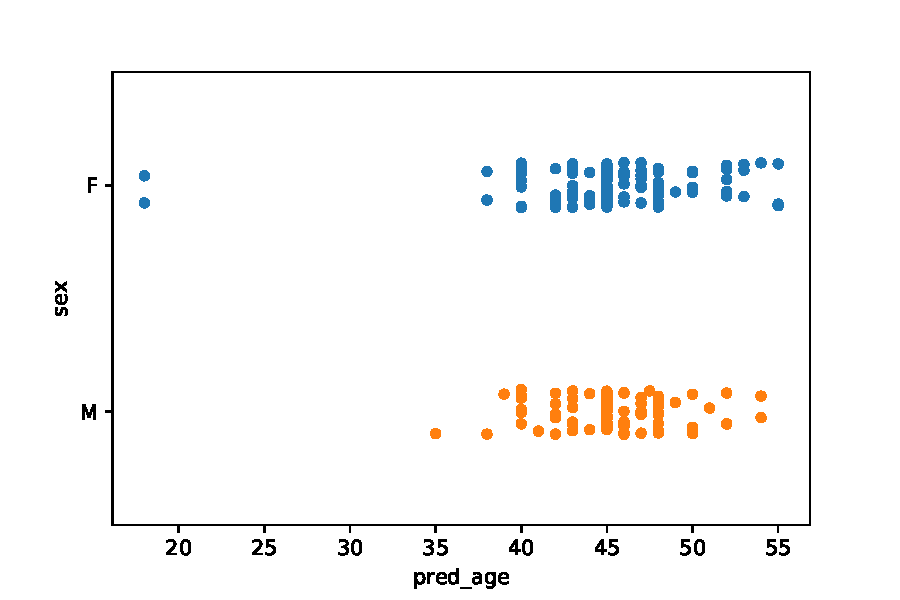
\includegraphics[width=0.7\textwidth]{sex.pdf}
	\caption{Age estimation distribution of genders. 
	The x-axis represents the estimated age, 
	and the y-axis represents genders. The difference does't exist among dots of different colors.\label{sex}}
\end{figure}


\section{Age}
Same as above, we have ANOVA test.
\begin{lstlisting}
	import scipy
	archive = {i:j['pred_age'].tolist() for i,j in raw.groupby('age')}
	scipy.stats.f_oneway(*archive.values())
\end{lstlisting}

The result is:
\begin{lstlisting}
	F_onewayResult(statistic=1.189127155588131, pvalue=0.291846925534072)
\end{lstlisting}

P-value is more than 0.05, so we can't reject the null hypothesis. The underlying mean age estimation of each of the several groups(ages) is the same. It can be seen in figure \ref{age}
\begin{figure}[htbp]
	\centering
	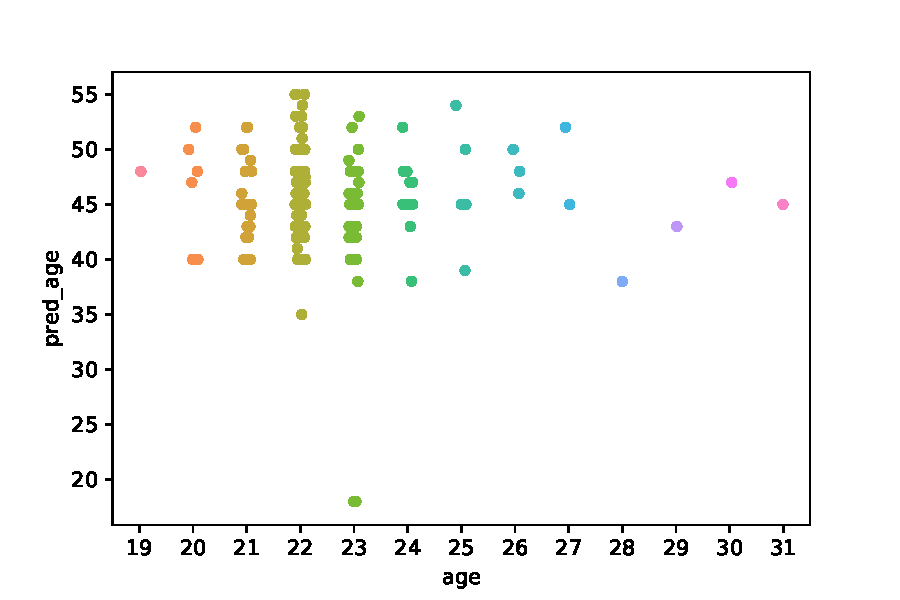
\includegraphics[width=0.7\textwidth]{age.pdf}
	\caption{Age estimation distribution of ages. 
	The x-axis represents the students' ages, 
	and the y-axis represents estimated age. The difference does't exist among dots of different colors.\label{age}}
\end{figure}




\chapter{Code}
My code is upload to \href{https://en.wikipedia.org/wiki/Pie_chart#Square_chart_/_Waffle_chart}{this repo}.

Statistical code:
\begin{lstlisting}
	'''
	@Description: 
	@Version: 
	@School: Tsinghua Univ
	@Date: 2019-09-19 09:59:30
	@LastEditors: Xie Yufeng
	@LastEditTime: 2019-09-22 23:52:45
	'''
	#!/usr/bin/env python
	# -*- encoding: utf-8 -*-
	'''
	@File    :   sta.py
	@Time    :   2019/09/19 09:59:37
	@Author  :   Xie Yufeng 
	@Version :   1.0
	@Contact :   xyfzkd@outlook.com
	@Desc    :   None
	'''
	
	# -*- coding: utf-8 -*-
	#%%
	import pandas as pd
	raw = pd.read_excel('raw.xlsx')
	
	#%%
	import seaborn as sns
	sns.set_style("darkgrid")
	#sns.set(style="ticks")
	g = sns.pairplot(raw,hue="sex",diag_kind='hist')
	
	#%%
	g.savefig('cov.pdf',facecolor='white')
	
	#%%
	from pywaffle import Waffle
	import pandas as pd
	import matplotlib.pyplot as plt
	#%%
	df_age = raw.groupby('age').size().reset_index(name='counts_age')
	n_categories = df_agef.shape[0]
	colors_age = [plt.cm.Set3(i/float(n_categories)) for i in range(n_categories)]
	fig = plt.figure(
		FigureClass=Waffle,
		plots={
			'111': {
				'values': df_age['counts_age'],
				'labels': ["{1}".format(n[0], n[1]) for n in df_age[['age', 'counts_age']].itertuples()],
				'legend': {'loc': 'upper left', 'bbox_to_anchor': (1.05, 1), 'fontsize': 12, 'title':'Age'},
				'title': {'label': '# Vehicles by Age', 'loc': 'center', 'fontsize':18},
				'colors': colors_age
			}
		},
		rows=12,
		figsize=(16, 10)
	)
	fig.savefig("waffe.pdf",transparent=True)
	#%%
	df_age = raw.groupby('sex').size().reset_index(name='counts_age')
	n_categories = df_age.shape[0]
	colors_age = [plt.cm.Set3(i/float(n_categories)) for i in range(n_categories)]
	fig = plt.figure(
		FigureClass=Waffle,
		plots={
			'111': {
				'values': df_age['counts_age'],
				'labels': ["{1}".format(n[0], n[1]) for n in df_age[['sex', 'counts_age']].itertuples()],
				'legend': {'loc': 'upper left', 'bbox_to_anchor': (1.05, 1), 'fontsize': 12, 'title':'Gender'},
				'title': {'label': '# Vehicles by Age', 'loc': 'center', 'fontsize':18},
				'colors': colors_age
			}
		},
		rows=12,
		figsize=(16, 10)
	)
	fig.savefig("waffle_sex.pdf",transparent=True)
	#%%
	df_agef = raw[raw['sex']=='F'].groupby('age').size().reset_index(name='counts_age')
	df_agem = raw[raw['sex']=='M'].groupby('age').size().reset_index(name='counts_age')
	n_categoriesf = df_agef.shape[0]
	n_categoriesm = df_agem.shape[0]
	colors_agef = [plt.cm.Set3(i/float(n_categoriesf)) for i in range(n_categoriesf)]
	colors_agem = [plt.cm.Set3(i/float(n_categoriesm)) for i in range(n_categoriesm)]
	fig = plt.figure(
		FigureClass=Waffle,
		plots={
			'211': {
				'values': df_agef['counts_age'],
				'labels': ["{1}".format(n[0], n[1]) for n in df_agef[['age', 'counts_age']].itertuples()],
				'legend': {'loc': 'upper left', 'bbox_to_anchor': (1.05, 1), 'fontsize': 12, 'title':'Age'},
				'title': {'label': '# Vehicles by Age', 'loc': 'center', 'fontsize':18},
				'colors': colors_agef
			},
			'212': {
				'values': df_agem['counts_age'],
				'labels': ["{1}".format(n[0], n[1]) for n in df_agem[['age', 'counts_age']].itertuples()],
				'legend': {'loc': 'upper left', 'bbox_to_anchor': (1.05, 1), 'fontsize': 12, 'title':'Age'},
				'title': {'label': '# Vehicles by Age', 'loc': 'center', 'fontsize':18},
				'colors': colors_agem
			}
		},
		columns=6,
		figsize=(16, 10)
	)
	#g.savefig('1.pdf',facecolor='white')
	#%%
	raw
	#%%
	from scipy import stats
	fig,ax = plt.subplots()
	scipy.stats.probplot(raw['pred_age'],dist='norm',plot=ax,fit=True)
	#%%
	import probscale
	def equality_line(ax, label=None):
		limits = [
			np.min([ax.get_xlim(), ax.get_ylim()]),
			np.max([ax.get_xlim(), ax.get_ylim()]),
		]
		ax.set_xlim(limits)
		ax.set_ylim(limits)
		ax.plot(limits, limits, 'k-', alpha=0.75, zorder=0, label=label)
	
	norm = stats.norm(loc=21, scale=8)
	fig, ax = plt.subplots(figsize=(5, 5))
	ax.set_aspect('equal')
	
	common_opts = dict(
		plottype='qq',
		probax='x',
		problabel='Theoretical Quantiles',
		datalabel='Emperical Quantiles',
		scatter_kws=dict(label='Bill amounts')
	)
	
	fig = probscale.probplot(raw['pred_age'], ax=ax, dist=norm, **common_opts)
	
	equality_line(ax, label='Guessed Normal Distribution')
	ax.legend(loc='lower right')
	sns.despine()
	#%%
	fig.savefig('norm.pdf',edgecolor='black',transparent=False)
	
	#%%
	import seaborn as sns
	import numpy as np
	x = np.linspace(min(raw['pred_age']), max(raw['pred_age']), 50)
	y = 239*1/(3.82 * np.sqrt(2 * np.pi))*np.exp( - (x - 45.12)**2 / (2 * 3.82**2))
	plt.plot(x,y)
	plt.hist(raw['pred_age'],bins=int(max(raw['pred_age'])-min(raw['pred_age'])))
	plt.savefig('normbin.pdf')
	#%%
	max(raw['pred_age'])-min(raw['pred_age'])
	
	#%%
	import seaborn as sns
	import numpy as np 
	import matplotlib.mlab as mlab 
	import matplotlib.pyplot as plt
	x = raw['pred_age']
	mu =np.mean(x)
	sigma =np.std(x,ddof=1)
	
	num_bins = int(max(raw['pred_age'])-min(raw['pred_age']))
	n, bins, patches = plt.hist(x, num_bins,normed=1, facecolor='blue', alpha=0.5) 
	y = mlab.normpdf(bins, mu, sigma)
	plt.plot(bins, y, 'r--')
	plt.xlabel('Age Estimation') #绘制x轴 
	plt.ylabel('Probability') #绘制y轴 
	plt.title(r'Normal Distribution Fit: $\mu=%.1f$,$\sigma=%.1f$'%(mu,sigma))
	plt.savefig('norm_fit.pdf')
	#%%
	def qqplot(sample=raw['pred_age']):
		import numpy as np
		x = sample
		mu =np.mean(x)
		sigma =np.std(x,ddof=1)
		from scipy.stats import norm,percentileofscore
		samp_pct = [percentileofscore(x, i) for i in x]
		fit_pct = [norm.cdf(i,mu,sigma)*100 for i in x]
		import matplotlib.pyplot as plt
		plt.scatter(x=samp_pct, y=fit_pct)
		linex = np.arange(0, 100, 1)
		liney = np.arange(0, 100, 1)
		plt.plot(linex, liney, 'r--')
		plt.xlabel('Sample Percentage%') #绘制x轴 
		plt.ylabel('Fit Percentage%') #绘制y轴 
		plt.title(r'Q-Q plot')
		plt.savefig('qqplot.pdf')
	qqplot()
	
	
	#%%
	import scipy.stats as stats
	x = raw['pred_age']
	mu =np.mean(x)
	sigma =np.std(x,ddof=1)
	normed_data=(x-mu)/sigma
	print(stats.kstest(normed_data,'norm'))
	#%%
	import scipy.stats as stats
	x = raw['pred_age']
	sp_x=x.tolist()
	sp_x.sort()
	sp_x = sp_x[2:]
	mu =np.mean(sp_x)
	sigma =np.std(sp_x,ddof=1)
	normed_data=(sp_x-mu)/sigma
	print(stats.kstest(normed_data,'norm'))
	
	#%%
	
	import scipy.stats as stats
	x = raw[raw['sex']=='M']['pred_age']
	mu =np.mean(x)
	sigma =np.std(x,ddof=1)
	normed_data=(x-mu)/sigma
	print(stats.kstest(normed_data,'norm'))
	#%%
	import scipy.stats as stats
	x = raw[raw['sex']=='F']['pred_age']
	sp_x=x.tolist()
	sp_x.sort()
	sp_x = sp_x[2:]
	mu =np.mean(sp_x)
	sigma =np.std(sp_x,ddof=1)
	normed_data=(sp_x-mu)/sigma
	print(stats.kstest(normed_data,'norm'))
	
	#%%
	import scipy.stats as stats
	import pandas as pd
	pd.DataFrame(raw.groupby('sex').describe()).to_csv('des_sex.csv',sep=',')
	pd.DataFrame(raw.groupby('age').describe()).to_csv('des.csv',sep=',')
	
	#%%
	from scipy import stats
	
	F, p = stats.f_oneway(d_data['ctrl'], d_data['trt1'], d_data['trt2'])
	#%%
	for i,j in raw.groupby('sex'):
		print(i)
	
	#%%
	[j for i,j in raw.groupby('sex')].values()
	
	#%%
	archive = {'group1': np.array([ 1, 2, 3 ]),
			'group2': np.array([ 9, 8, 7])}
	
	#%%
	
	
	#%%
	import scipy
	archive = {i:j['pred_age'].tolist() for i,j in raw.groupby('sex')}
	scipy.stats.f_oneway(*archive.values())
	
	#%%
	import seaborn as sns
	import matplotlib.pyplot as plt
	fig,ax = plt.subplots()
	ax = sns.stripplot(y='sex',x='pred_age',data=raw)
	fig.savefig('sex.pdf')
	#%%
	import scipy
	archive = {i:j['pred_age'].tolist() for i,j in raw.groupby('age')}
	scipy.stats.f_oneway(*archive.values())
	
	#%%
	import seaborn as sns
	import matplotlib.pyplot as plt
	fig,ax = plt.subplots()
	ax = sns.stripplot(x='age',y='pred_age',data=raw)
	fig.savefig('age.pdf')
	
	
	#%%
	
\end{lstlisting}

\end{document}
